\question \textbf{Array with fixed sized elements}

Given the following sequence of integers: $A = \left[8, 11, 40, 53, 32, 33, 16, 18\right]$.

\begin{parts}
\part Transform the integers into their binary representation with an appropriate number of bits $l$.

\begin{solution}
    
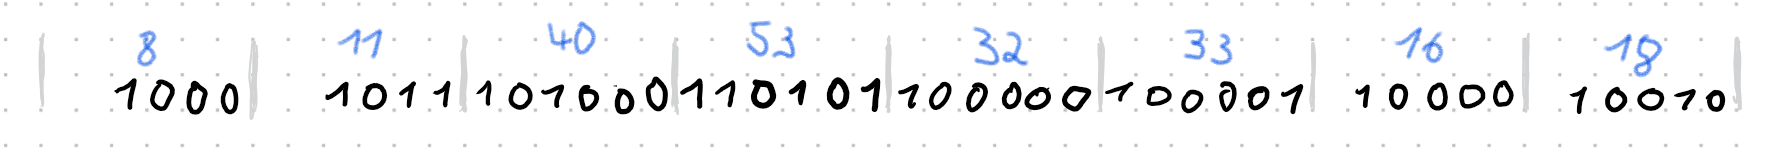
\includegraphics[width=0.8\linewidth]{task_1/a1_1.png}
\end{solution}

\part Write down the virtual bitvector $B$ representing the integer array $A$ (see figure 3.2 on slide 2031+1)

\begin{solution}
    
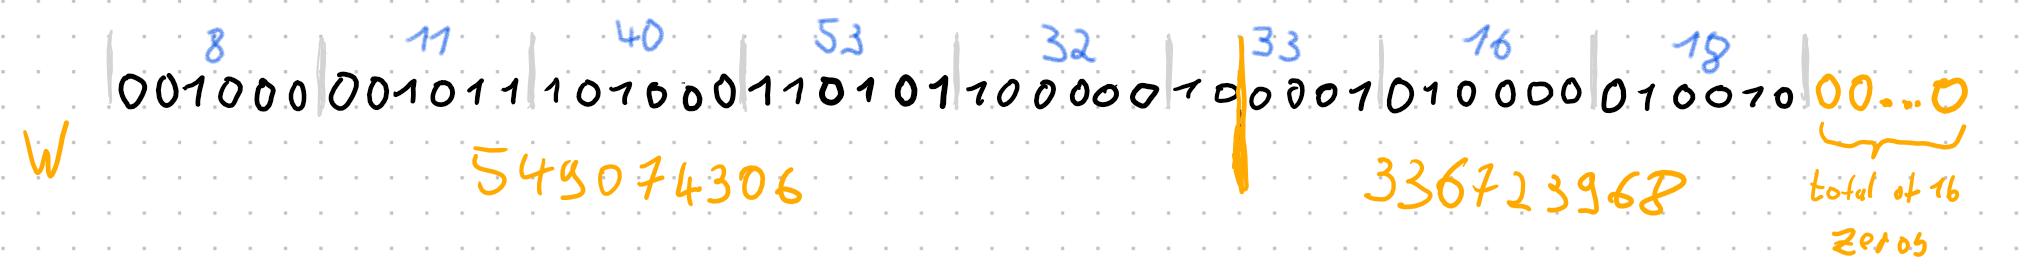
\includegraphics[width=0.8\linewidth]{task_1/a1_2.png}
\end{solution}

\part Write down the integer array $W$ that stores the virtual bitvector $B$ in an 32-bit integer array.

\begin{solution}
    
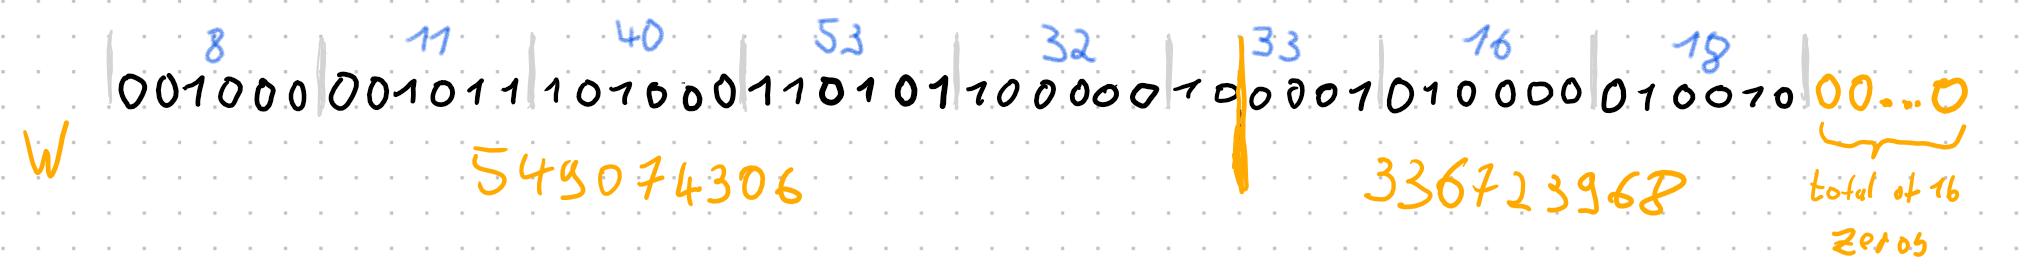
\includegraphics[width=0.8\linewidth]{task_1/a1_3.png}
\end{solution}

\part How do you access $B[8]$?

\begin{solution}

\textit{We assume that the task asks for \enquote{How do you access $A[8]$ using $B$}}
\begin{equation*}
\begin{aligned}
A[i]&=B[(i-1)l+1, il] \\
A[8]&=B[(8-1)6+1, 8\cdot6]=B[43,48]
\end{aligned}
\end{equation*}


\end{solution}

\part Write down how you would read $A[2] = 11$ given only $W$.

\begin{solution}

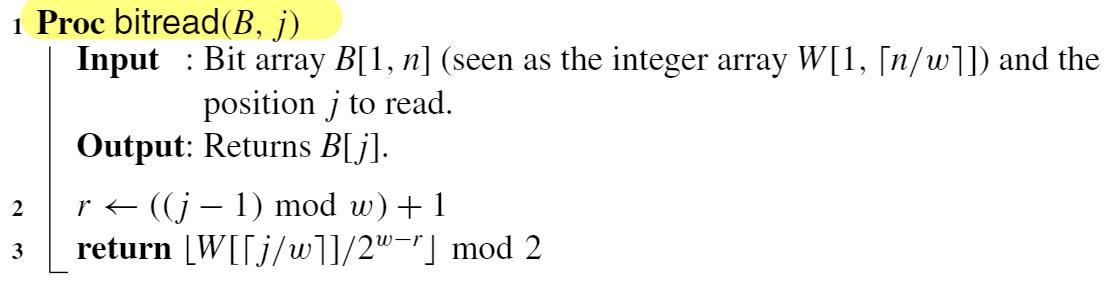
\includegraphics[width=0.7\linewidth]{task_1/bitread_w.png}

    
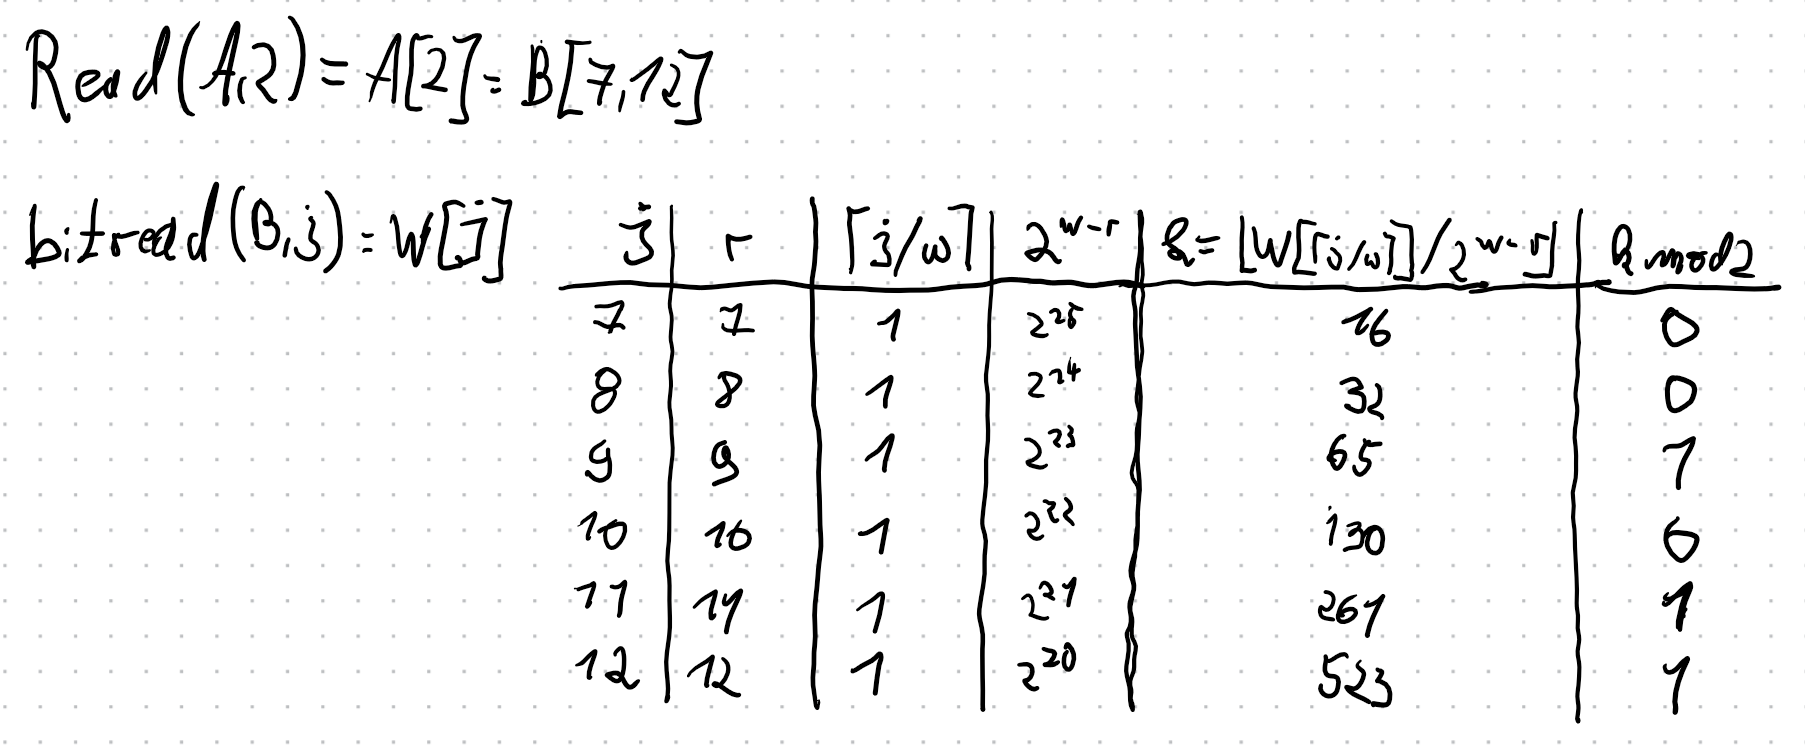
\includegraphics[width=0.8\linewidth]{task_1/a1_5.png}
\end{solution}

\part Write down how you would read $A[6] = 33$ given only $W$.

\begin{solution}
    
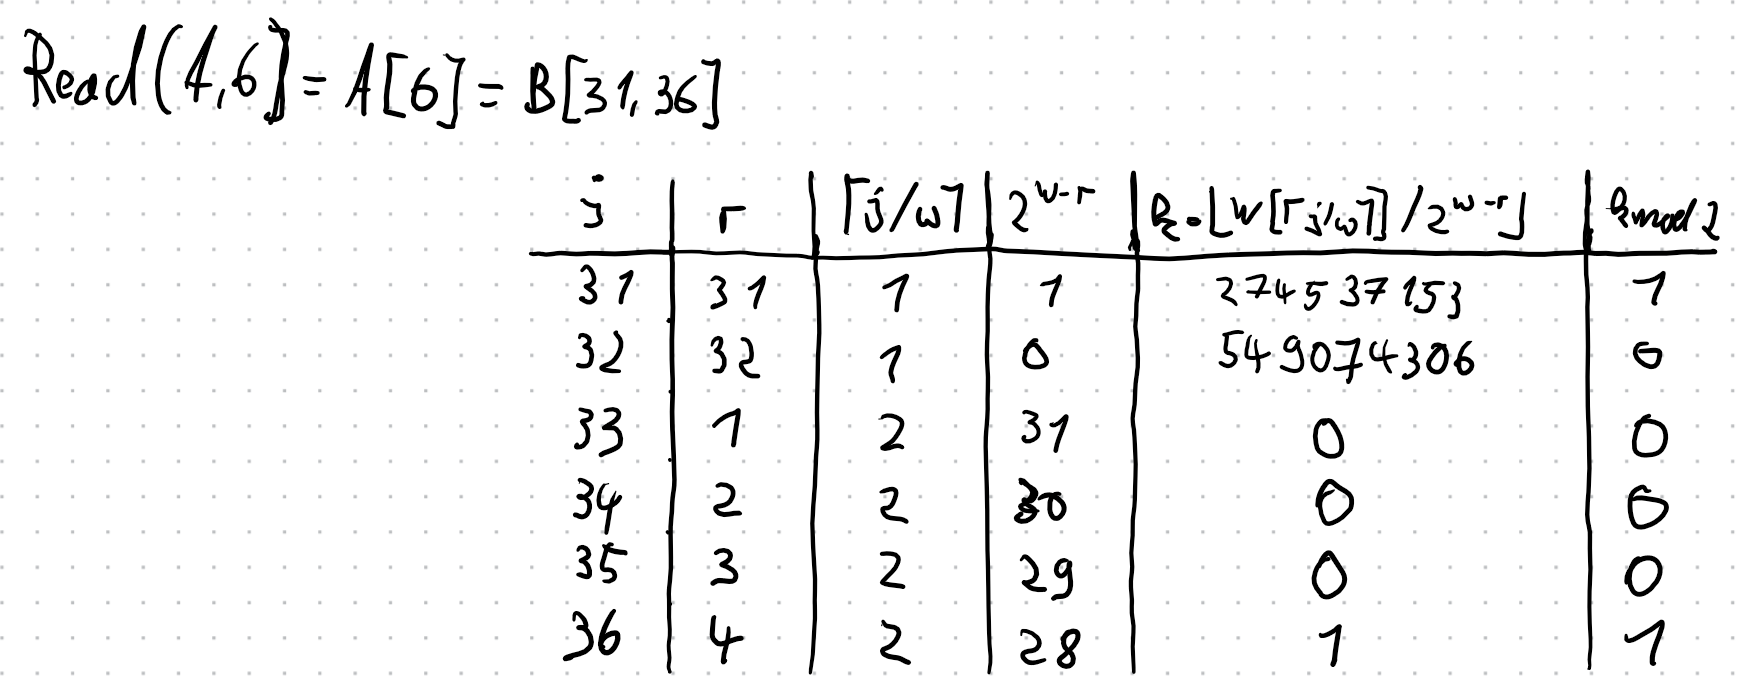
\includegraphics[width=0.8\linewidth]{task_1/a1_6.png}
\end{solution}

\part How many bits do you need to store array $A$?

\begin{solution}

$8\cdot 6=48$Bits
\end{solution}


\end{parts}


% For tasks without simply remove the \begin{parts}...\part...\end{parts} commands